\section{Integral}
\begin{theorem}[Hauptsatz der Integralrechnung] Angenommen $f:[a, b] \to \R$ ist stetig, dann definieren wir
\begin{align*}
	F(x) &= \int_a^x f(t) \, dt \\
	F'(x) &= f(x) \hspace{1cm} \forall \, x \in [a, b]
\end{align*}
\end{theorem}

\begin{corollary}[Stammfunktion] Jede stetige Funktion auf einem kompakten Intervall $[a,\; b]$ hat eine Stammfunktion.
\[
	\int_a^b f(x) \; dx = F(b) - F(a)
\]
\end{corollary}

\begin{corollary}[Linearität] Es gilt:
\[
	\int \alpha f(x) + \beta g(x)\,dx = \alpha \int f(x)\,dx + \beta \int g(x)\,dx
\]
\end{corollary}

\begin{definition}Falls $a < b$ ist und $f$ auf $[a, b]$ integrierbar ist, dann definieren wir:
\[
	\int_b^a f(x) \; dx = - \int_a^b f(x) \; dx
\]
\end{definition}
\newpage
\subsection{Integral-Berechnung}
\subsubsection{Substitutionsregel}
Unbestimmt: $\int f(g(x)) \, g'(x) \, dx = \int f(u) \, du$ mit $u = g(x)$\\
Bestimmt: $\int_a^b f(g(x)) \, g'(x) \, dx = \int_{g(a)}^{g(b)} f(u) \, du$ mit $u = g(x)$

\begin{enumerate}
	\item Aufstellen der Substitutionsgleichungen:\\
	$u = g(x)$ und $ \frac{du}{dx} = g'(x) \Leftrightarrow du = g'(x) \, dx$ $\Leftrightarrow$ $dx = \frac{du}{g'(x)}$

	\item Durchführen der Substitution:\\
	Man ersetzt also $u = g(x)$ und $du = g'(x) \, dx$ oder $dx = \frac{du}{g'(x)}$, wobei um $dx$ zu ersetzen die erste Variante besser ist, da so auch noch $g'(x)$ aus dem Integral entfernt wird. \\
	Wenn noch $x$ übrig sind im Integral, ist ein Zwischenschritt nötig:
	Löse $u = g(x)$ nach $x$ auf, somit resultiert eine neue Formel mit 
	$x = h(u)$, substituiere nun $x$ durch $h(u)$.

	\item Berechnen des neuen Integrals nach $u$:\\
	Bei bestimmten Integralen: Sei $\int_a^b \ldots \,dx$. Dann sind die neuen
	Grenzen für das neue Integral $g(a)$ und $g(b)$

	\item Rücksubstitution:\\
	Ersetze im Ergebnis $u$ wieder mit $g(x)$. \\
	Merke: Bei einem bestimmten Integral, kann auf die Rücksubstitution verzichtet werden, wenn man die Integrationsgrenzen mitsubstituiert hat!
\end{enumerate}

\textbf{Substitutionstips:}
{\small
\begin{itemize}
	\item $\int f(ax + b) \; dx$ verwende $u = ax + b$
	\vspace{0.1cm}
	
	\item $\int f(x) \cdot f'(x) \; dx$ verwende $u = f(x)$\\
	Falls die Ableitung von $f$ ganz oder fast im Term steht!
	\vspace{0.1cm}
	
	\item $\int f(x)^n \cdot f'(x) \; dx$ verwende $u = f(x)$
	\vspace{0.1cm}

	\item $\int \frac{f'(x)}{f(x)} \; dx$ verwende $u = f(x)$\\
	Falls die Ableitung von $f$ ganz oder fast im Zähler steht!
	\vspace{0.1cm}

	\item $\int f(g(x)) \cdot g'(x) \; dx$ verwende $u = g(x)$
	\vspace{0.1cm}
	
	\item Integrale die $\sqrt{a^2 - x^2}$ enthalten: $u = a^2 - x^2$ oder\\
	$x = a \cdot \sin(u) $ und $dx = a \cdot \cos(u) \, du$ und $\sqrt{a^2 - x^2} = a \cdot \cos(u)$
	\vspace{0.1cm}

	\item Integrale die $\sqrt{a^2 + x^2}$ enthalten: $u = a^2 + x^2$ oder\\
	$x = a \cdot \sinh(u) $ und $dx = a \cdot \cosh(u) \, du$ und $\sqrt{a^2 + x^2} = a \cdot \cosh(u)$

	\vspace{0.1cm}
	\item Integrale die $\sqrt{x^2 - a^2}$ enthalten: $u = x^2 - a^2$ oder\\
	$x = a \cdot \cosh(u) $ und $dx = a \cdot \sinh(u) \, du$ und $\sqrt{x^2 - a^2} = a \cdot \sinh(u)$
\end{itemize}
\textbf{Bsp:} $\int \sqrt{1 + x^2} \; dx$\\
Wir verwenden die Substitution: $x = \sinh(u)$ mit $a = 1$. Daraus folgt aus $\frac{dx}{du}: dx = \cosh(u)$. 
Nun vollziehen wir die Substitution und erhalten: $\int \sqrt{1 + \sinh(u)^2} \cdot \cosh(u) \; du$
Aus der Formelsammlung entnehmen wir $\sqrt{a^2 + x^2} = \cosh(x)$ und ersetzen also diesen Term zu:  
$\int \cosh(u)^2 \; du$. Für diesen Typ haben wir nun in der Formelsammlung eine konkrete Lösung und es lässt sich nun leicht integrieren. Merke: Diese Ersetzungen können alle aus den Tips entnommen werden!
}

\subsubsection{Beispiel: Substitution}
$\int_0^2 x \sqrt{x+1}^3 \,dx$

Die Wurzel wird substituiert: $u = g(x) = \sqrt{x+1}$.

\begin{enumerate}[itemsep=0.5em]
	\item $\frac{du}{dx} = g'(x) = \frac{1}{2\sqrt{x+1}} = \frac{1}{2u}$. Somit
	wird $\sqrt{x+1}^3$ durch $u^3$ ersetzt und $dx$ durch
	$2u\,du$. Im Integral wären somit die Wurzel und das
	$dx$ ersetzt. Es bleibt noch das $x$ übrig vor der Wurzel. Lösen wird
	$\sqrt{x+1} = u$ nach $x$ auf, so erhalten wir $x = u^2 - 1$.
	\item Neue Grenzen: $g(0) = 1$ und $g(2) = \sqrt{3}$
	\item $\int_0^2 x \sqrt{x+1}^3 \,dx = \int_1^{\sqrt{3}} (u^2 - 1)u^3 2u \,du =
	2\int(u^6 -u^4) \,du = [\frac{2}{7}u^7 - \frac{2}{5}u^5]_{1}^{\sqrt{3}}$
	\item Rücksubstitution: $\int_0^2 x \sqrt{x+1}^3 \,dx =
	[\frac{2}{7}\sqrt{x+1}^7 - \frac{2}{5}\sqrt{x+1}^5]_{0}^{2} = \ldots = \frac{144}{35}\sqrt{3} +
	\frac{4}{35}$
\end{enumerate}

\subsubsection{Partielle Integration}
Die Formel für die Partielle Integration lautet:
\[
	\int u(x) \cdot v'(x) \, dx = u(x) \cdot v(x) - \int u'(x) \cdot v(x) \, dx
\]

In vielen Fällen lässt sich das Integral $\int f(x) \, dx$ wie folgt lösen.
\begin{enumerate}
	\item Man zerlegt $f(x)$ in geeigneter Weise in ein Produkt so dass $f(x) = u(x) \cdot v'(x)$ gilt. Man legt also einfach fest welcher Teil von $f$ dem $u$ und welcher Teil dem $v'$ entspricht (ohne dabei $f$ zu verändern!). Wähle u so, dass die Ableitung möglichst simpel ist (Bsp. $u$ = ein Polynom) damit das Integral einfacher wird.

	\item Berechne $u'$ und $v$ um es in obige Formel einzusetzen und dann das Integral zu bilden.
\end{enumerate}
Bsp: $\int \ucomment{u}{x} \, \ucomment{v'}{\cos(x)} = x \sin(x) - \int 1 \cdot \sin(x) = x \sin(x) + \cos(x) + C$\\
\textbf{Tip:} Wenn $f(x)$ aus einem Produkt mit Polynomen besteht, muss man meist das Polynom ableiten (Also u = Polynom). Eventuell mehrmals partiell integrieren. Bei jeder partiellen Integration wird so das Polynom um 1 verringert! 

\subsubsection{Allgemeine Tips}
\begin{itemize}[leftmargin=*]
	\item Hat man einen Bruch und Grad im Zähler $\geq$ Grad im Nenner. Führe immer eine Polynomdivision durch. Nun kann meist direkt ein einfacheres Resultat integriert werden. Falls immer noch zu kompliziert, siehe nächster Punkt.

	\item Hat man komplizierten Bruch und Grad im Zähler $<$ Grad im Nenner, hilft oft eine Partialbruchzerlegung.

	\item Integral mit $e^x,sin,cos$ wie: $\int_0^{\pi/2} \sin(x) \cos(2x)$ muss oft 2x partiell integriert werden und dann mit Startintegral gleichsetzen! (Wähle $v'$ so, dass Integral ohne Bruch entsteht)

	\item Integralgrenzen können aufschluss über Substitution geben.

	\item Oft ist besser Wurzel als Polynome aufzufassen, $\sqrt{x} = x^{1/2}$
\end{itemize}

% nicht relevant
%\subsubsection{Integrale mit Parametern}
%	Sei $h: \R^2 \to \R$ stetig und partiell nach $t$ diffbar mit stetiger Ableitungsfunktion. Betrachte 
%	\[ u(y) = \int_0^y h(x,y) \; \rmd x \]
%	Dann ist $u \in C^1(\R)$ und für die Ableitung gilt
%	\[ \dot{u}(y) = h(x,y)|_{x=y} + \int_0^y \frac{\partial h}{\partial y} (x,y) \; \rmd x \]

% Beispiel zu trivial
%\subsubsection{Beispiel: einfaches Integral}
%Das Integral $\int_{-2}^1 x^2 \,dx$ berechnet die blaue Fläche die durch die Funktion $f(x) = x^2$ beschränkt wird.
%$F(x)$ sei die Stammfunktion von $f(x)$,  generell berechnen wir $\int x^y \,dx = \frac{x^{(y+1)}}{y+1}$, somit $F(x) = \frac{x^3}{3}$.
%Somit $\int_{-2}^1 x^2 \,dx = F(x) \left |_{-2}^1 \right. = F(1) - F(-2) =  \frac{1^3}{3} -  \frac{-2^3}{3} = \frac{1}{3} +  \frac{8}{3} = 3.$

%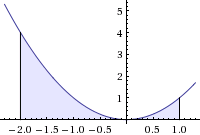
\includegraphics[scale=0.5]{integral_x2.png}

\subsection{Uneigentliche Integrale}
\begin{definition}[Uneigentliches Integral] Sei $f: \; [a, b[ \to \R$ eine Funktion. So ist das uneigentliche Integral, im Falle der Konvergenz, definiert durch (Analog für ($g: \; ]a, b] \to \R$):
\begin{align*}
	\int_a^b f(x) \; dx = \lim_{\beta \to b^-} \int_a^{\beta} f(x)\; dx\\
	\int_a^b g(x) \; dx = \lim_{\alpha \to a^+} \int_{\alpha}^{b} g(x)\; dx
\end{align*}
\end{definition}

Vorgehen:
\begin{enumerate}
	\item Kritische Stelle (Bsp. $\infty$) durch eine Variable ersetzen und Grenzwert gegen den vorherigen Wert streben lassen.

	\item Betrachte es wie ein bestimmtes Integral und berechne das Integral für die neuen Grenzen aus. 

	\item Anschliessend den Grenzwert berechnen um zu sehen, gegen welchen Wert das Resultat strebt. Wenn der Grenzwert existiert ($\neq \pm \infty$), konvergiert also das Integral und man hat das uneigentliche Integral ausgerechnet. Ansonsten divergiert der Grenzwert und somit auch das Integral
\end{enumerate}
%\vspace{-0.3cm}
{\small
\hspace{-0.35cm}
\textbf{Beispiel:}
\vspace{-0.2cm}
\begin{align*}
	\hspace{-0.35cm} \int_{a}^{\infty} f(x) \; dx = \lim_{b \to \infty} \int_a^b f(x) \; dx = \lim_{b \to \infty} \Bigl[ F(x) \Bigr]_a^b = \lim_{b \to \infty} [F(b) - F(a)] = \dots
\end{align*}}\textbf{Merke:} \\
Wenn das unbestimmte Integral innerhalb der Integralsgrenzen an einer Stelle nicht definiert oder nicht stetig ist, muss das Integral in zwei separate uneigentliche Integrale aufgeteilt werden mit dieser Stelle als Intervallsgrenze! \\

{\small
\hspace{-0.35cm}
\textbf{Beispiel:}
\vspace{-0.2cm}
\begin{align*}
	\hspace{-0.35cm} \int_{-2}^{2} \frac{1}{x} \; dx = \int_{-2}^{0} \frac{1}{x} \; dx + \int_{0}^{2} \frac{1}{x} \; dx = \lim_{b \to 0^-} \int_{-2}^{b} \frac{1}{x} \; dx + \lim_{a \to 0^+} \int_{a}^{2} \frac{1}{x} \; dx = \dots
\end{align*}}



